\documentclass[11pt,a4paper]{ctexart}
\usepackage{fontspec}
\defaultfontfeatures{Mapping=tex-text}
\usepackage{xunicode}
\usepackage{xltxtra}
%\setmainfont{???}
\usepackage{amsmath}
\usepackage{amsfonts}
\usepackage{amssymb}
\usepackage{graphicx}
\usepackage{amsthm}
\usepackage{array}
\usepackage{float}   %{H}
\usepackage{booktabs}  %\toprule[1.5pt]
\usepackage[titletoc]{appendix}
\usepackage{tcolorbox} %彩色框框
%===================%插入代码需要的控制
\usepackage{listings}
\usepackage{listings}
\usepackage{xcolor}
\setmonofont{Consolas}%字体
\lstset{
	numbers=left, 
	numberstyle= \tiny, 
	keywordstyle= \color{ blue!70},
	commentstyle= \color{red!50!green!50!blue!50}, 
	frame=shadowbox, % 阴影效果
	rulesepcolor= \color{ red!20!green!20!blue!20} ,
	escapeinside=``,% 英文分号中可写入中文
	breaklines=true,
	basicstyle=\ttfamily 
} 
%===================%
\usepackage[left=2cm,right=2cm,top=2cm,bottom=2cm]{geometry}

\newtheorem{theorem}{定理}
\newtheorem{definition}{定义}
\newtheorem*{solution}{解}

\title{定性数据统计分析作业 (3)}
\author{钟瑜 \quad 222018314210044}
\date{\today}
\begin{document}
\maketitle
\pagestyle{plain}%设置页码
%==================================================================================%
\begin{figure}[H]
	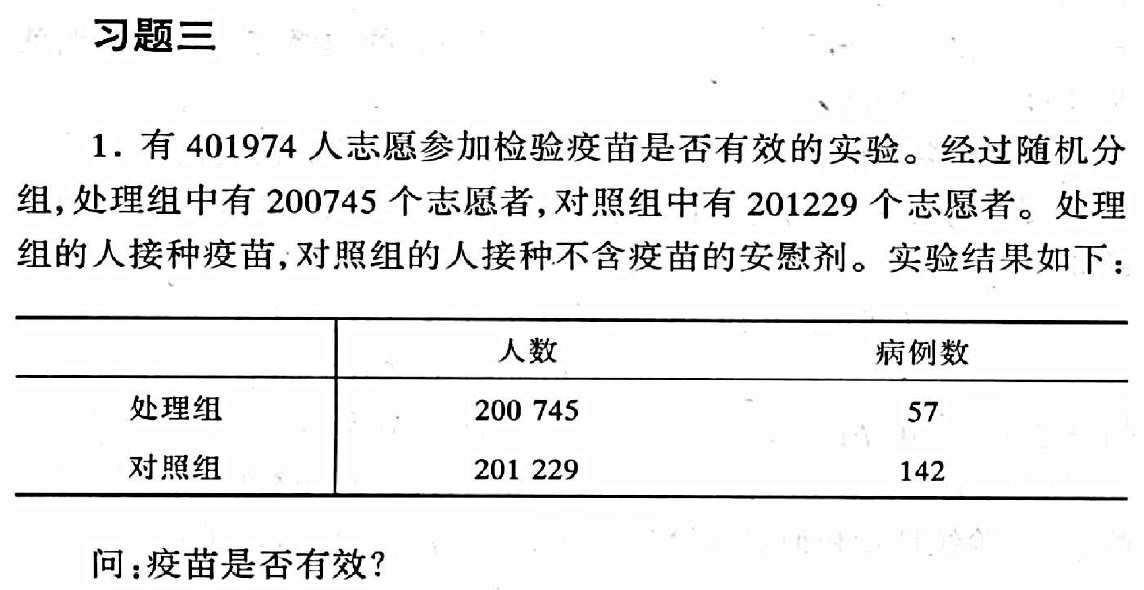
\includegraphics[width=0.7\textwidth]{1.png}
\end{figure}
\begin{solution}
四格表如下所示:
\begin{table}[!htbp]   %[H]
	\centering
	\begin{tabular}{cccc}
		\toprule[1.5pt]
		 & 无疾病$ (B) $ & 有疾病$(\bar{B})$ & 合计\\
		\midrule[1pt]
		处理组(有疫苗)$ (A) $ & 200603 & 142 & 200745\\
		对照组(无疫苗)$(\bar{A})$ & 201172  & 57 & 201229\\
		\midrule[1pt]
		合计 & 401775 & 199 & 401974\\
		\bottomrule[1.5pt]
	\end{tabular}
\end{table}
%%%%%%%%%%%%%%%%%%%%%%%%%%%%%%%%
%\begin{table}[!htbp]   %[H]
%	\centering
%	\begin{tabular}{cccc}
%		\toprule[1.5pt]
%		& 有疾病(B) & 无疾病($\bar{B}$) & 合计\\
%		\midrule[1pt]
%		处理组(有疫苗)(A) & $ p_{11}= $0.0003532567 & $ p_{12}= $0.4990447143 & $ p_{1+}= $0.499397971\\
%		对照组(无疫苗)($ \bar{A} $) & $ p_{21}= $0.0001418002 & $ p_{22}= $0.5004602288& $ p_{2+}= $0.500602029\\
%		\midrule[1pt]
%		合计 & $ p_{+1}= $0.0004950569 & $ p_{+2}= $0.9995049431 & 1\\
%		\bottomrule[1.5pt]
%	\end{tabular}
%\end{table}
%%%%%%%%%%%%%%%%%%%%%%%%%%%%%%%%%%%
显然为一个单侧给定的四格表,要看疫苗是否有效,需要对四格表进行检验.如果疫苗有效,那么有属性A的个体中有属性B的比例高.

\end{solution}

1.无方向检验
\begin{lstlisting}[language=r]
> x<-matrix(c(200688,201087,57,142),nrow=2)
> chisq.test(x,correct = F)

Pearson's Chi-squared test

data:  x
X-squared = 36.12, df = 1, p-value = 1.855e-09
\end{lstlisting}
p值小于$ \alpha $=0.001,故否定原假设,疫苗注射与否与患病与否相关.\\

2.有方向检验(备择假设为:有属性A的个体中有属性B的比例高)
\begin{lstlisting}[language=r]
> x<-matrix(c(200688,201087,57,142),nrow=2)
> fgtest_1=function(x)
+   {
	+   U=sqrt(sum(x))*(x[1]*x[4]-x[2]*x[3])/sqrt(((x[1]+x[2])*(x[3]+x[4])*(x[1]+x[3])*(x[2]+x[4])))  #卡方统计量
	+     p_value=pnorm(-U);p_value
	+     }
> fgtest_1(x)
[1] 9.276332e-10
\end{lstlisting}
p值小于$ \alpha $=0.001,故否定原假设,认为有属性A的个体中有属性B的比例高,即注射疫苗后无疾病的比例更高,疫苗有效.\\


3.有方向检验(备择假设为:有属性A的个体中有属性B的比例低)
\begin{lstlisting}[language=r]
> fgtest_2=function(x)
+ {
	+   U=sqrt(sum(x))*(x[1]*x[4]-x[2]*x[3])/sqrt(((x[1]+x[2])*(x[3]+x[4])*(x[1]+x[3])*(x[2]+x[4]))) 
	+   p_value=pnorm(U);p_value
	+ }
> fgtest_2(x)
[1] 1
\end{lstlisting}
p值大于$ \alpha $=0.001,肯定原假设,认为有属性A的个体中有属性B的比例高,即注射疫苗后无疾病的比例更高,疫苗有效.


\end{document}